\documentclass{beamer}
%\usetheme{Frankfurt}  %% Themenwahl
\usetheme[height=7mm]{Boadilla}
\usefonttheme{structuresmallcapsserif} 
\usepackage[utf8x]{inputenc}
\usecolortheme{crane} 
%\useinnertheme{umbcboxes}
%------------------------------------------------------
\title{Kolloqium}
\subtitle{Entwicklung eines Systems zur
			  Entfernungsabschätzung für
			  Phasen basiertes UHF 
			  RFID Tracking durch 
			  Verwendung evolutionärer
			  Berechnungsverfahren}
\author{Christoph Gnip}
\date{\today}
%------------------------------------------------------

%------------------------------------------------------
\newtheorem{fazit}{Fazit} 
%------------------------------------------------------


%------------------------------------------------------
\begin{document}
%------------------------------------------------------
\maketitle
\frame{\tableofcontents}

%------------------------------------------------------
\section{Einleitung}
\subsection{Motivation}
\begin{frame} %%Eine Folie
  \frametitle{Motivation}
  
  	Tabelle mit Gegenüberstellung verschiedener Verfahren.
  	
\end{frame}

\newtheorem{fazit}{Fazit} 


\subsection{Grundlagen}
\begin{frame} %%Eine Folie
  \frametitle{Mathematische Grundlagen}
  	- Mathematische Optimierung
	- Evolutionäre verfahren
	- CMA-ES
\end{frame}

\begin{frame} %%Eine Folie
  \frametitle{Physikalische Grundlagen}
	- Funk basierende Messung auf dem RFID-Standard 
	- Phasenmessung
\end{frame}

\subsection{Grundlage2n}
\begin{frame} %%Eine Folie
  \frametitle{Test}
  \begin{test} %%Definition
    Beschreibung des Problems
  \end{test}
\end{frame}

%------------------------------------------------------
\section{Lösung}
\subsection{Modellierung}
%\begin{frame}
%  \frametitle{Modellierung} %%Folientitel
%%  \begin{definition} %%Definition
%%    Ergebnisse hier...
%%  \end{definition}
%\end{frame}
%------------------------------------------------------
\begin{frame}
  \frametitle{Anforderungen}
%
\begin{itemize} 
  \pause 
  \item Auf der Basis der Trilateration
  \item Lineares Modell zur Entfernungsberechnung
  \item Einsetzbar als Objektfunktion
\end{itemize} 
	
%
\end{frame}
%------------------------------------------------------
\begin{frame}
  \frametitle{Modellierung  1}
%
  \begin{center}
	\tiny Skizze der Szene mit einem Tag und drei Antennen. Als Referenzpunkt dient eine Landmarke, später eine Antenne.
%
  	\includegraphics[width=.7\textwidth]{../img/trilaterationScene.pdf}
  \end{center}
\[
r_k^2= (x_k-x)^2 + (y_k-y)^2 + (z_k-z)^2
\]
\end{frame}
%------------------------------------------------------
\begin{frame}
  \frametitle{Modellierung  1}
%
  \begin{center}
	\tiny Skizze der Szene mit einem Tag und drei Antennen. Als Referenzpunkt dient eine Landmarke, später eine Antenne.
%
  	\includegraphics[width=.7\textwidth]{../img/trilaterationScene_mono.pdf}
  \end{center}
\[
r_k^2= (x_k-x)^2 + (y_k-y)^2 + (z_k-z)^2
\]
\end{frame}
%------------------------------------------------------
%\begin{frame}
%  	\frametitle{Modellierung 2}
%%  
%	Wir notieren:
%%	
%	\begin{align}
%		r_1^2&= (x_1-x )^2 + (y_1-y )^2 + (z_1-z )^2\\
%		r_2^2&= (x_2-x )^2 + (y_2-y )^2 + (z_2-z )^2\\
%		r_3^2&= (x_3-x )^2 + (y_3-y )^2 + (z_3-z )^2\\
%		\nonumber\\
%		r_0^2&= (x_0-x )^2 + (y_0-y )^2 + (z_0-z )^2\\
%		\nonumber\\
%		r_{0k}^2&= (x_0-x_k )^2 + (y_0-y_k )^2 + (z_0-z_k )^2 \\
%		\nonumber\\
%		r(\Theta_k,n_k)&=\frac{\lambda}{2}\left(\Theta_k+n_k\right)
%%		
%	\end{align}
%%
%\end{frame}
%------------------------------------------------------
\begin{frame}
  	\frametitle{Modellierung 3}
%--
	Gleichung der Form:
	\[\mathbf{A}\mathbf{x}=\mathbf{b}\]  
%--
	,wobei:
	\begin{multline}
	\mathbf{A}=\\
	\left(
		\begin{array}{cccccccccc}
			x_1-x_0 & y_1-y_0 & z_1-z_0 & -a_1 & 0 & 0 & -a_2\Theta_0 & a_2\Theta_1 & 0 & 0 \\
			x_2-x_0 & y_2-y_0 & z_2-z_0 & 0 & -a_1 & 0 & -a_2\Theta_0& 0 & a_2\Theta_2 & 0 \\
			x_3-x_0 & y_3-y_0 & z_3-z_0 & 0 & 0 & -a_1 & -a_2\Theta_0& 0 & 0 & a_2\Theta_3
		\end{array}
	\right) \nonumber
	\end{multline}
%--
	und
	\begin{multline}
	\mathbf{x}=\\
	\left(
		\begin{array}{cccccccccc}
			x-x_0 & y-y_0 & z-z_0 &	n_0^2-n_1^2	& \dots	& n_0^2-n_3^2 & n_0 & n_1 & \dots &	n_3	
		\end{array}
	\right)^T\nonumber
	\end{multline}
%--
	\begin{multline}
		\mathbf{b}=\\
		\left(
			\begin{array}{c}
				a_{0k}-a_{3kj} 
			\end{array}
			\right)^T
			= c_{kj}'\nonumber
		\end{multline}
%--		
\end{frame}
%------------------------------------------------------
\begin{frame}
%
  	\frametitle{Modell - Zusammenfassung}
  	\begin{itemize}
		\item Ermöglicht Positionsberechnung durch vier beliebige Antennen 
		\item Kann eine eindeutige Lösung liefern
		\item Als Objektfunktion für evol. Optimierung geeignet*
		\item 'Vertauschen' erlaubt Bestimmung der Antennenposition
  	\end{itemize}
%  	
\end{frame}
%------------------------------------------------------
\subsection{Implementation}
\begin{frame}
%
  	\frametitle{Implementation}
%  	
	\begin{textblock*}{8cm}(4cm,2.5cm) % {block width} (coords)
		\centering
  		\includegraphics[width=7cm]{../img/PRPSEvolutionImplementation.pdf}
%  		\footnote{Grafik entnommen aus \url{http://en.wikipedia.org/w/index.php?title=File:Concept_of_directional_optimization_in_CMA-ES_algorithm.png&oldid=532567533}}
  	\end{textblock*}
%  	
	\begin{textblock*}{4cm}(0cm,2cm) % {block width} (coords)
  			\begin{itemize}
  				\item Parallel zur PRPS-Software
  				\item Plattform\-unabhängig
   				\item Einfaches Interface
   				\item Nahtlose Implementation
  		  	\end{itemize}
  	\end{textblock*}
  
%  	
\end{frame}
%------------------------------------------------------
\section{Ergebnisse}
%\subsection{Künstliche Messwerte}
%%------------------------------------------------------
%\begin{frame}
%  \frametitle{Ergebnisse}
%  \begin{center}
%  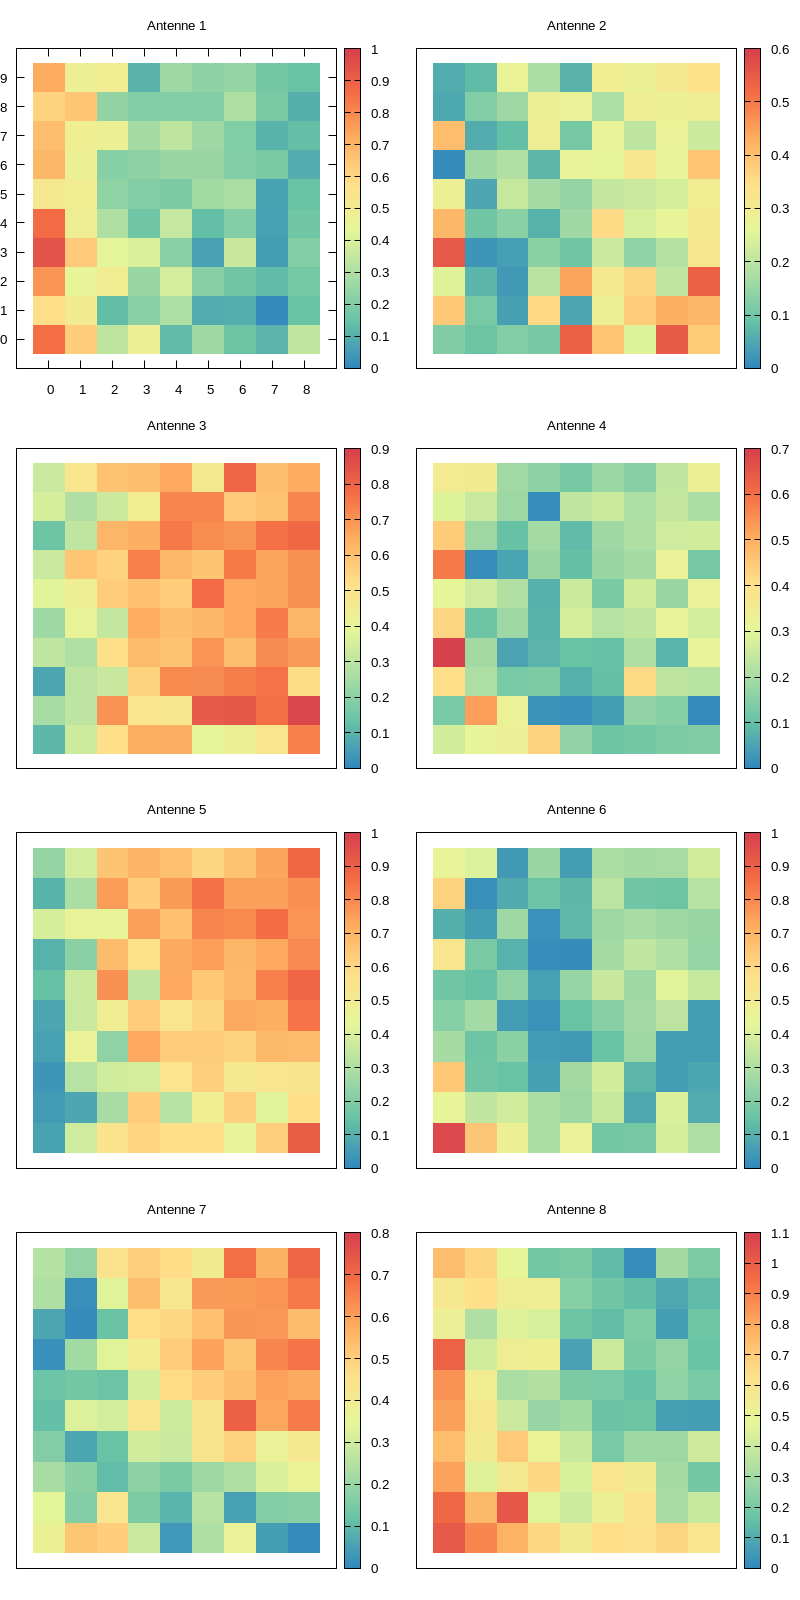
\includegraphics[width=.3\textwidth]{../img/result.png}
%  \qquad
%  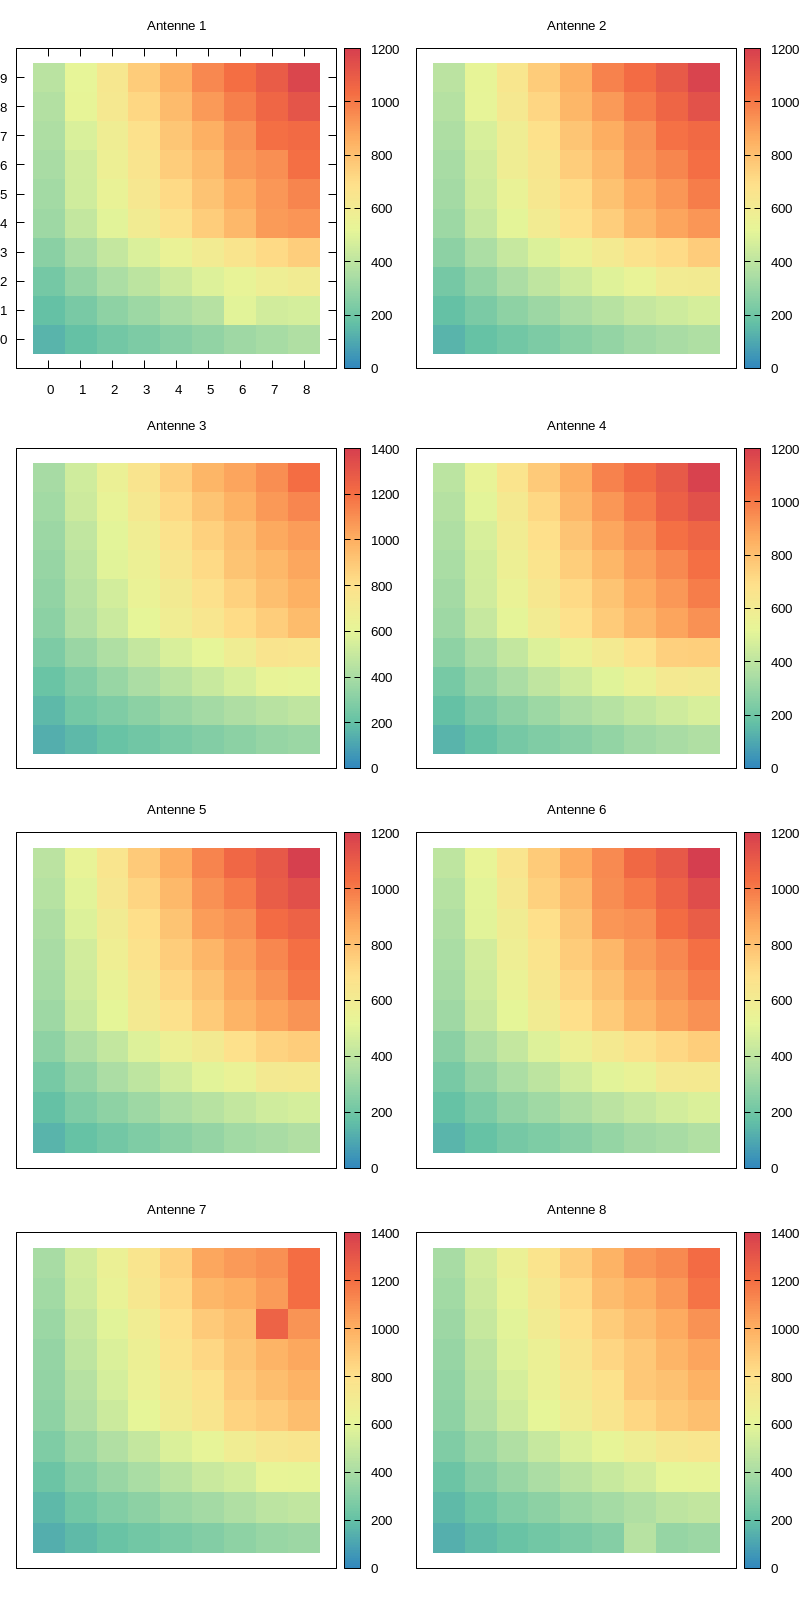
\includegraphics[width=.3\textwidth]{../img/resultstiming.png}
%  \end{center}
%\end{frame}
%------------------------------------------------------
\subsection{Reale Messwerte}
%------------------------------------------------------
\begin{frame}
  \frametitle{Optimierungsverlauf}
  \begin{center}
  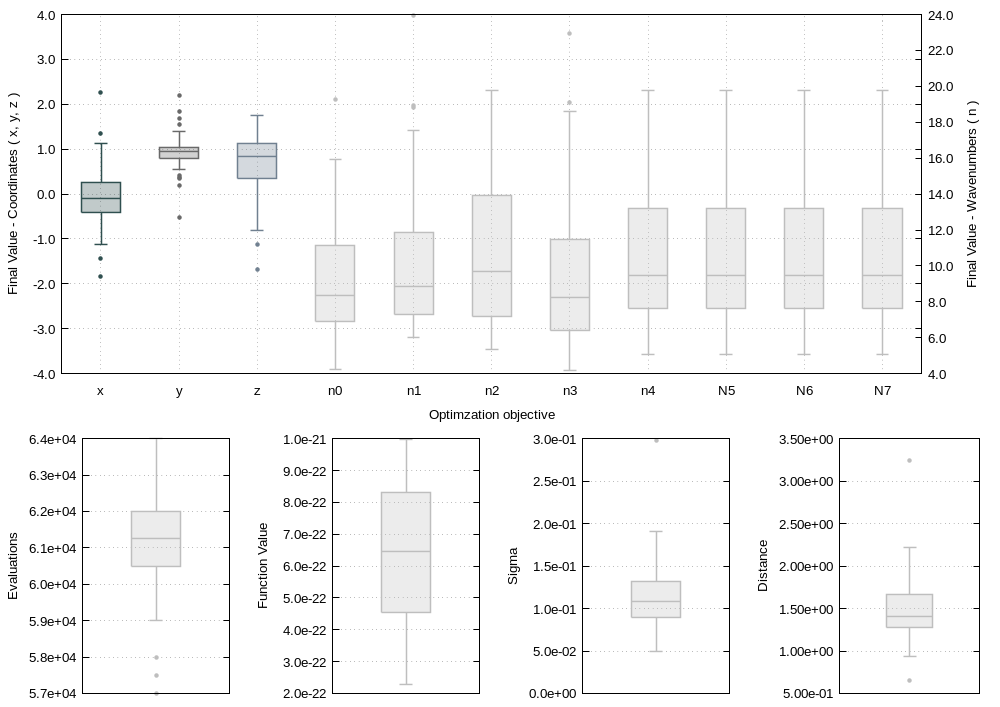
\includegraphics[width=.47\textwidth]{../img/boxes2089.png}
  \qquad
  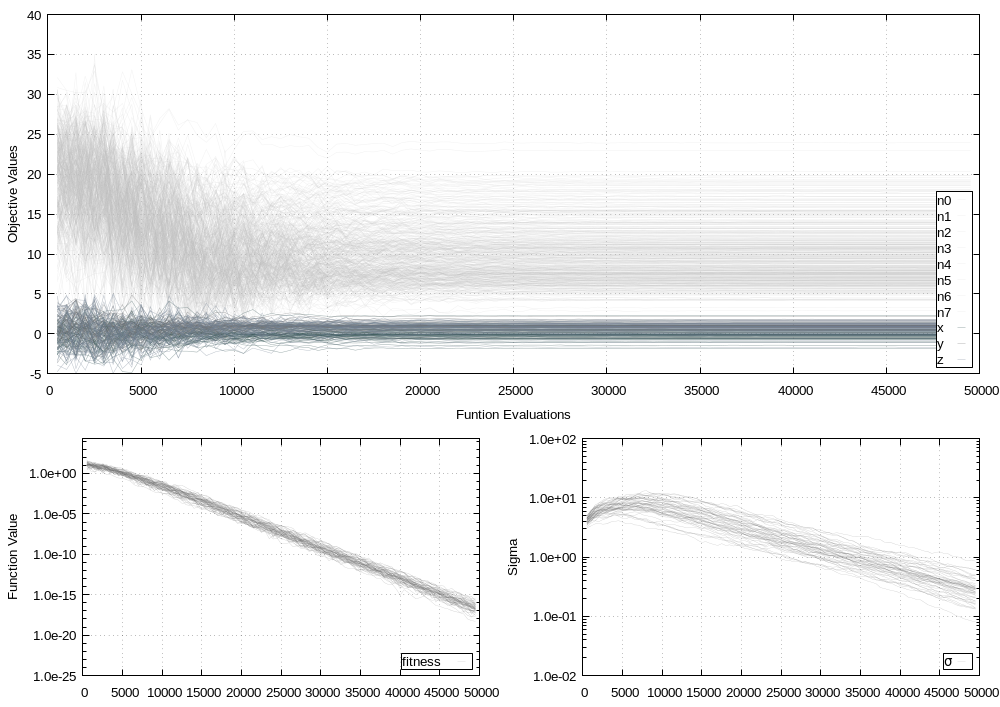
\includegraphics[width=.47\textwidth]{../img/lines2089.png}
  \end{center}
\end{frame}
%------------------------------------------------------
\begin{frame}
  \frametitle{Ergebnisse}
  \begin{center}
  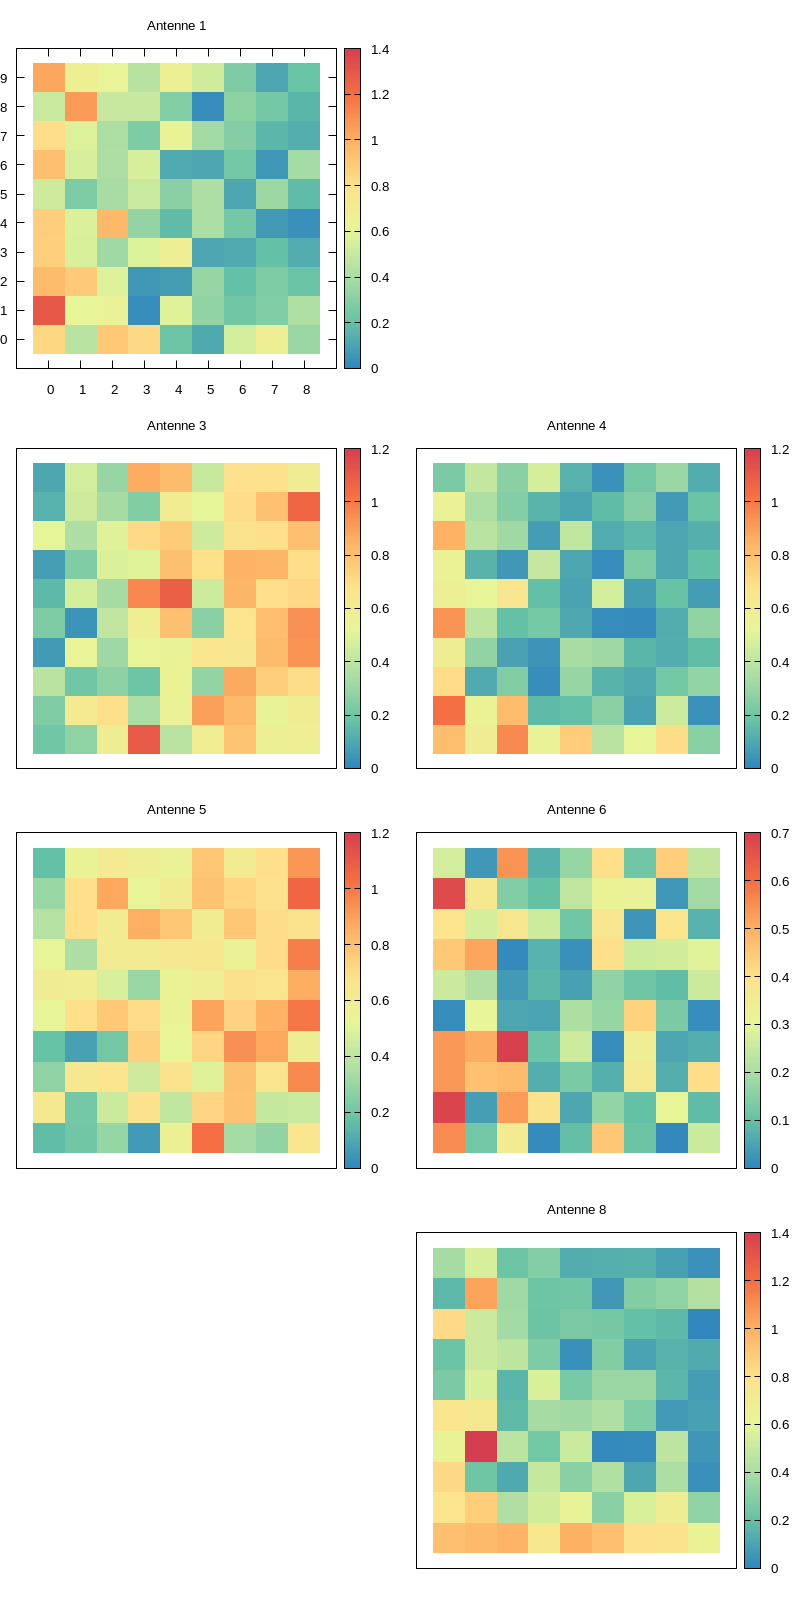
\includegraphics[width=.3\textwidth]{../img/resultRealData.png}
  \qquad
  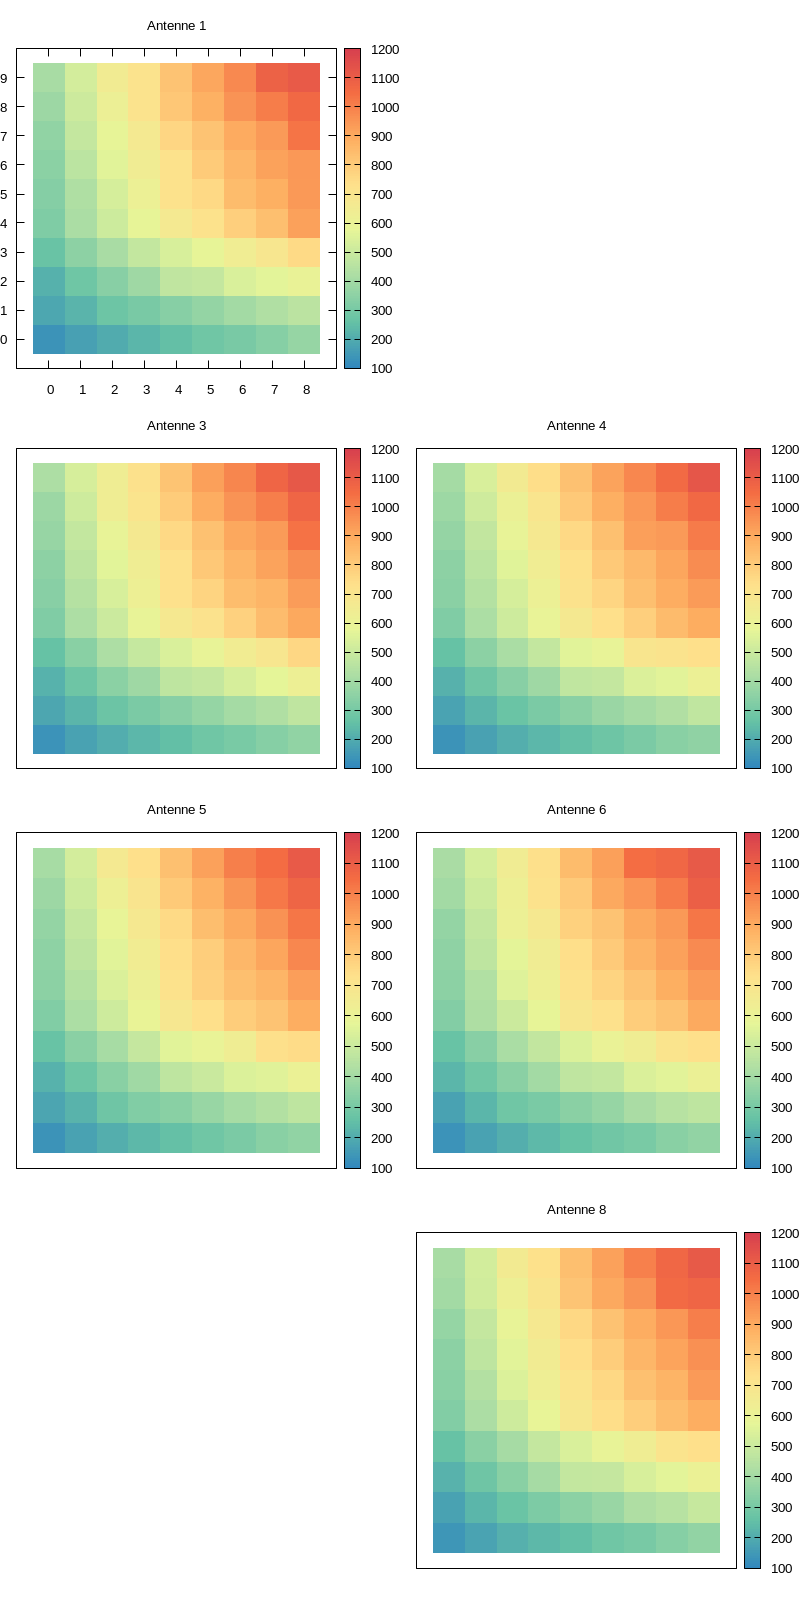
\includegraphics[width=.3\textwidth]{../img/resultstimingreal.png}
  \end{center}
\end{frame}

%------------------------------------------------------
%------------------------------------------------------
\section{Fazit}
\begin{frame} %%Eine Folie
  \frametitle{Fazit} %%Folientitel
  \begin{definition} %%Definition
    Fazit hier...
  \end{definition}
\end{frame}
%------------------------------------------------------
\end{document}

%Cg2to187gc@gmX